This section describes the purpose, use and intended user audience for the L-Tunes laser harp. L-Tunes is a laser-based digital instrument and MIDI device that uses lasers to trigger a note when the laser is blocked or obstructed. The device can be used to play sounds like an harp, with presets and parameters to emulate other instruments and sounds. Users of L-Tunes will be able to play the device like an instrument and even create new sounds via built in sound generators. This product is intended for anyone, but particularly musicians, harp-enthusiasts, and children. 

\subsection{Purpose and Use}
The L-Tunes laser harp should be used to play sounds like a harp, along with being a versatile MIDI device that can be used to trigger sounds in a DAW (Digital Audio Workstation). 

\subsection{Intended Audience}
This device can be used by anyone, however the device is intended to be used by musicians, harp-enthusiasts, and young children. This device is designed for  anyone looking for an alternative to a real harp with strings. Users who are unable to play a harp due to physical ailments such as carpal tunnel, as the device does not require any pressure to be applied to trigger sound. 

\begin{figure}[h!]
	\centering
   	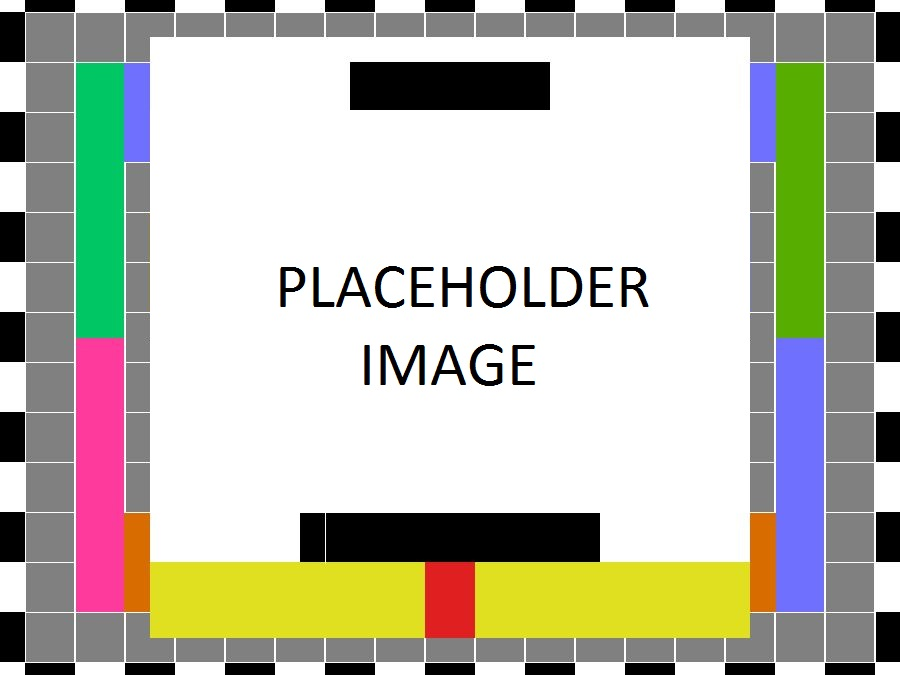
\includegraphics[width=0.60\textwidth]{images/test_image}
    \caption{X conceptual drawing}
\end{figure}
